\documentclass[border=20pt]{standalone}
\renewcommand\familydefault{\sfdefault} % Default family: serif
\usepackage{tikz}
\usetikzlibrary{calc}
\usetikzlibrary{shapes.geometric}
\usetikzlibrary{arrows.meta,arrows}
\usetikzlibrary{positioning}
\tikzset{
  initial/.style={circle, fill},
  decision/.style={diamond, black, draw},
  action/.style={rectangle, draw, rounded corners},
  arrow/.style={draw, -{Latex[length=3mm]}, thick}
  }
\begin{document}
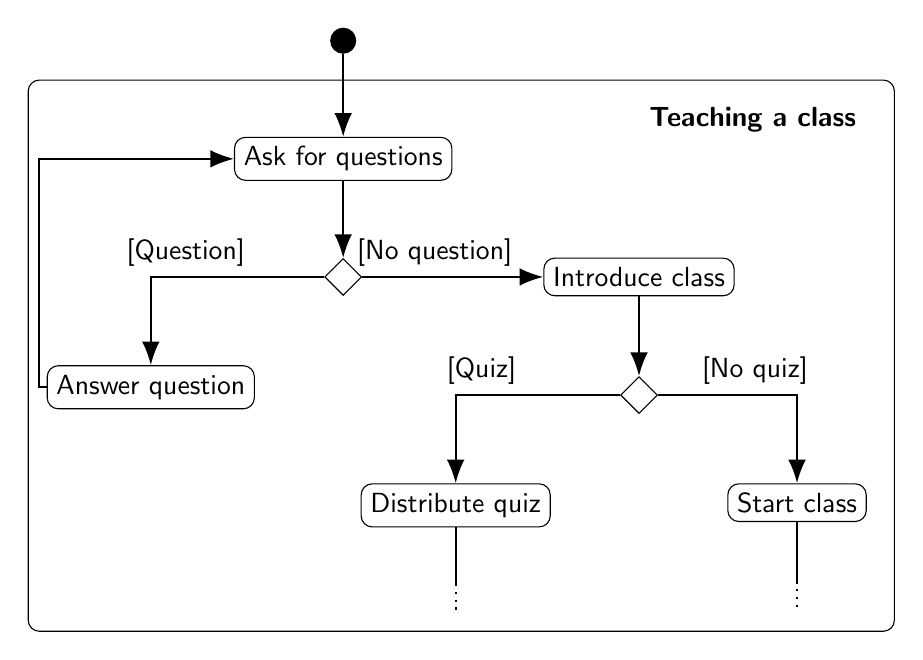
\begin{tikzpicture}[node distance=1.5cm]
	% Frame
	\draw [rounded corners] (-4,-1.5) rectangle (7, -8.5);
	\node (title) at (5.2, -2) {\textbf{Teaching a class}};

	% Nodes
	\node[initial] (initial) at (0,-1) {};
	\node[action, below of = initial] (ask)  {Ask for questions};
	\node[decision, below of= ask] (decision1)  {};
	\node[action, below left = 1cm and 1cm of decision1] (answer) {Answer question};
	\node[action, right = 2.3cm of decision1] (intro) {Introduce class};
	\node[decision, below of=intro] (decision2)  {};
	\node[action, below left = 1cm and 1cm of decision2] (quiz) {Distribute quiz};
	\node[action, below right = 1cm and 1cm of decision2] (class) {Start class};

	% Arrow
	\draw [arrow] (initial) -- (ask);
	\draw [arrow] (ask) -- (decision1);
	\draw [arrow] (decision1) -- node[above, pos=1pt]{[Question]} ++(-2cm, 0) -| (answer);
	\draw [arrow] (answer.west) --  ++(-0.1, 0) -- ++(0, 2.8) |- (ask);
	\draw [arrow] (decision1) -- node[above, pos=.4pt]{[No question]} (intro);
	\draw [arrow] (intro) -- (decision2);
	\draw [arrow] (decision2) -- node[above, pos=1pt]{[Quiz]} ++(-2cm, 0) -| (quiz);
	\draw [arrow] (decision2) -- node[above, pos=.7pt]{[No quiz]} ++(2cm, 0) -| (class);

	% Etc.
	\draw[thick] (quiz) -- ++(0, -1);
	\draw[dotted, thick] ($ (quiz)+(0,-1)$) -- ++(0, -.33);
	\draw[thick] (class) -- ++(0, -1);
	\draw[dotted, thick] ($ (class)+(0,-1)$) -- ++(0, -.33);
\end{tikzpicture}
\end{document}

